\chapter{Trace Encoder Output Packets} \label{packets}

The bulk of this section describes the payload of packets output from the Trace Encoder.  
The infrastructure used to transport these packets is outside the scope of this document, and
as such the manner in which packets are encapsulated for transport is not specified.
However, the following information must be provided to the encapsulator:

\begin{itemize}
  \item The packet type;
  \item The packet length, in bytes;
  \item The packet payload.
\end{itemize}

Two example transport schemes are the UltraSoC Messaging Infrastructure, and the Arm Trace Bus.
Figure~\ref{fig:packet-format} shows the encapsulation used for the UltraSoC infrastructure:
\begin{itemize}
  \item The header byte contains a 5-bit field specifying the payload length in bytes, a 2-bit
    field indicating the "flow" (destination routing indicator), and a bit to indicate whether
    an optional 16-bit timestamp is present;
  \item The index field indicates the source of the packet.  The number of bits is system dependent,
    And the initial value emitted by the trace encoder is zero (it gets adjusted as it propagates 
    through the infrastructure);
  \item An optional 2-byte timestamp;
  \item The packet payload.
\end{itemize}

\begin{figure}[h]
  \begin{center}
    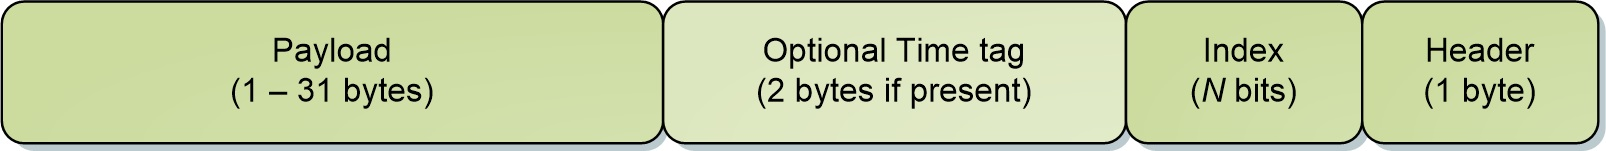
\includegraphics[height=1cm, width=9cm]{newPacket.jpg}
    \caption{Example encapsulated packet format}
    \label{fig:packet-format}
  \end{center}
\end{figure}


Alternatively, for ATB, the source of the packet is indicated by the \textbf{ATID} bus field, and there is
no equivalent of "flow", so an example encapsulation might be:
\begin{itemize}
  \item A 5-bit field specifying the payload length in bytes
  \item A bit to indicate whether an optional 16-bit timestamp is present;
  \item An optional 2-byte timestamp;
  \item The packet payload.
\end{itemize}
It may be desirable for packets to start aligned to an ATB word, in which the \textbf{ATBYTES} bus field
in the last beat of a packet can be used to indicate the number of valid bytes.

The remainder of this section describes the contents of the payload
portion which should be independent of the infrastructure.  In each table, the fields are listed in
transmission order: first field in the table is transmitted first, and multi-bit fields are 
transmitted LSB first.

This packet payload format is used to output encoded instruction
trace.  Three different formats are used according to the needs of the
encoding algorithm. The following tables show the format of the
payload - i.e. excluding any encapsulation.

In order to achieve best performance, actual packet lengths may be adjusted using 'sign based compression'.
At the very minimum this should be applied to the address field of format 1 and 2 packets, but ideally will 
be applied to the whole packet, regardless of format.  This technique eliminates identical bits from the most 
significant end of the packet, and adjusts the length of the packet accordingly.  A decoder receiving this 
shortened packet can reconstruct the original full-length packet by sign-extending from the most significant
received bit.  

Where the payload length given in the following tables, or after applying sign-based compression, is not a 
multiple of whole bytes in length, the payload must be sign-extended to the nearest byte boundary.

Whilst offering maximum encoding efficiency, variable length packets can present some challenges,
specifically in terms of identifying where the boundaries between packets occur either when packed
packets are written to memory, or when packets are streamed offchip via a communications channel.  Two 
potential solutions to this are as follows:

\begin{itemize}
  \item If the maximum packet payload length is 2\textsuperscript{N}-1 (for example, if N is 5, then the maximum length is
    31 bytes), and the minimum packet payload length is 1, then a sequence of at least 2\textsuperscript{N} zero 
    bytes cannot occur within a packet payload, and therefore the first non-zero byte seen after a sequence of 
    at least 2\textsuperscript{N} zero bytes must be the first byte of a packet.  This approach can be used for
    alignment in either memory or a data stream;
  \item An alternative approach suitable for packets written to memory is to divide memory into blocks of M bytes
    (e.g. 1kbyte blocks), and write packets to memory such that the first byte in every block is always the first
    byte of a packet.  This means packets cannot span block boundaries, and so zero bytes must be used to pad between 
    the end of the last message in a block and the block boundary.
\end{itemize}

\section{Format 3 packets} \label{sec:format3}

Format 3 packets are used for synchronization, reporting context and supporting information.  There are 4
sub-formats.

Throughout this document, the term "synchronization packet" is used.  This refers specifically to format 3, 
subformat 0 and subformat 1 packets.

\section{Format 3 subformat 0 - Synchronisation} \label{sec:format30}

This packet contains all the information the decoder needs to fully identify an instruction.  It is sent for
the first traced instruction (unless that instruction also happens to be a the first in an exception handler), 
and when resynchronization has been scheduled by expiry of the resynchronisation timer.

\begin{table}[htp]
  \centering
  \caption{Packet format 3, subformat 0}
  \label{tab:te_inst3}
  \begin{tabulary}{\textwidth}{|l|p{35mm}|p{90mm}|}
    \hline
    {\bf Field name} & {\bf Bits} & {\bf Description} \\
    \hline
    \textbf{format} & 2 & 11 (sync): synchronisation\\
    \hline
    \textbf{subformat} & 2 & 00 (start): Start of tracing, or resync \\
    \hline
    \textbf{branch} & 1 & Set to 0 if the address points to a branch instruction, and the branch was taken.  
              Set to 1 if the instruction is not a branch or if the branch is not taken. \\
    \hline
    \textbf{privilege} & \textit {privilege\_width\_p} & 
                The privilege level of the reported instruction\\
    \hline
    \textbf{context} &  \textit {context\_width\_p}, 
               or 0 if \textit {nocontext\_p} is 1 & 
               The instruction context \\
    \hline
    \textbf{address} & \textit {iaddress\_width\_p - iaddress\_lsb\_p} & 
              Full instruction address.  Address alignment is determined by \textit {iaddress\_lsb\_p} Address must be left shifted in order to recreate original byte address. \\
    \hline
  \end{tabulary}
\end{table}

\subsection{Format 3 \textbf{branch} field}

This bit indicates the taken/not taken status in the case where the reported address points to a branch instruction.
Overall efficiency would be slightly improved if this bit was removed, and the branch status was instead 
"carried over" and reported in the next \textit{te\_inst} packet.  This was considered, but there are several
pathological cases where this approach fails.  Consider for example the situation where the first traced instruction
is a branch, and this is then followed immediately by an exception.  This results in format 3 packets being generated 
on two consecutive instructions.  The second packet does not contain a branch
map, so there is no way to report the branch status of the 1st branch, apart from by inserting a format 1 packet in 
between.  There are two issues with this:

\begin{itemize}
  \item It would require the generation of 2 packets on the same cycle, which adds significant additional complexity
    to the encoder;
  \item It would complicate the algorithm shown in figure~\ref{fig:algo}. 
\end{itemize}

\FloatBarrier
\section{Format 3 subformat 1 - Exception} \label{sec:format31}

This packet also contains all the information the decoder needs to fully identify an instruction.
It is sent following an exception, and as well as reporting the address of the exception handler, it also 
includes the exception cause and the address of the faulted instruction.

If the implicit exception mode is enabled (see section~\ref{sec:implicit-exception}), the address is omited.

\begin{table}[htp]
  \centering
  \caption{Packet format 3, subformat 1}
  \label{tab:te_inst3}
  \begin{tabulary}{\textwidth}{|l|p{35mm}|p{90mm}|}
    \hline
    {\bf Field name} & {\bf Bits} & {\bf Description} \\
    \hline
    \textbf{format} & 2 & 11 (sync): synchronisation\\
    \hline
    \textbf{subformat} & 2 & 01 (exception): Exception cause and trap handler address.\\
    \hline
    \textbf{branch} & 1 & Set to 0 if the address points to a branch instruction, and the branch was taken.  
              Set to 1 if the instruction is not a branch or if the branch is not taken. \\
    \hline
    \textbf{privilege} & \textit {privilege\_width\_p} & 
                The privilege level of the reported instruction.\\
    \hline
    \textbf{context} &  \textit {context\_width\_p}, 
               or 0 if \textit {nocontext\_p} is 1 & 
               The instruction context. \\
    \hline
    \textbf{ecause} & \textit {ecause\_width\_p} & 
             Exception cause. \\
    \hline
    \textbf{interrupt} & 1 & 
                Interrupt. \\
    \hline
    \textbf{address} & \textit {iaddress\_width\_p - iaddress\_lsb\_p} & 
              Full instruction address.  Address alignment is determined by \textit {iaddress\_lsb\_p} Address must be left shifted in order to recreate original byte address. \\
    \hline
    \textbf{tvalepc} & \textit {iaddress\_width\_p} & 
           Exception address if \textbf{ecause} is 2 and \textbf{interrupt} is 0 (illegal instruction exception), or trap value otherwise.\\
    \hline
  \end{tabulary}
\end{table}

\subsection{Format 3 \textbf{tvalepc} field}

This field reports the address of illegal instructions, or the trap value otherwise.  This ensures that
the address of the faulting instruction is reported for all required cases.  The trap value 
is set to the address of the faulting instruction for hardware breakpoints, access or page faults and 
instructions, loads or stores that are mis-aligned, but not for illegal instructions (for which it is set to the opcode).

\FloatBarrier
\section{Format 3 subformat 2 - Context} \label{sec:format32}

This packet contains only the context, and is output when the context changes and can be reported imprecisely (see Table~\ref{tab:context-type}).

\begin{table}[htp]
  \centering
  \caption{Packet format 3, subformat 2}
  \label{tab:te_inst3}
  \begin{tabulary}{\textwidth}{|l|p{35mm}|p{90mm}|}
    \hline
    {\bf Field name} & {\bf Bits} & {\bf Description} \\
    \hline
    \textbf{format} & 2 & 11 (sync): synchronisation\\
    \hline
    \textbf{subformat}  & 2 & 10 (context): Context change \\
    \hline
    \textbf{privilege} & \textit {privilege\_width\_p} & 
                The privilege level of the new context.\\
    \hline
    \textbf{context} &  \textit {context\_width\_p} & The instruction context. \\
    \hline
  \end{tabulary}
\end{table}

\section{Format 3 subformat 3 - Support} \label{sec:format33}

This packet provides supporting information to aid the decoder.  It is issued when

\begin{itemize}
  \item Trace is enabled or disabled;
  \item The operating mode changes;
  \item One or more trace packets cannot be sent (for example, due back-pressure from the packet transport infrastructure).
\end{itemize}

The \textbf{options} field is a placeholder that must be replaced by an implementation specific set of individual bits - one for each of the
optional modes supported by the encoder.

\begin{table}[htp]
  \centering
  \caption{Packet format 3, subformat 3}
  \label{tab:te_inst3}
  \begin{tabulary}{\textwidth}{|l|p{35mm}|p{90mm}|}
    \hline
     {\bf Field name} & {\bf Bits} & {\bf Description} \\
     \hline
     \textbf{format} & 2 & 11 (sync): synchronisation\\
     \hline
     \textbf{subformat}  & 2 & 11 (support): Supporting information for the decoder \\
     \hline
     \textbf{enable} & 1 & Indicates if the encoder is enabled\\
     \hline
     \textbf{encoder\_mode} & N & Identifies trace algorithm\newline
       Details and number of bits implementation dependent.  Currently Branch trace is the only mode defined, indicated by the value 0.\\
     \hline
     \textbf{qual\_status} & 2 & Indicates qualification status\newline
       00 (no\_change): No change to filter qualification \newline
       01 (ended\_rep): Qualification ended, preceding \textbf{te\_inst} sent explicitly to indicate last qualification instruction\newline
       10: (trace\_lost): One or more packets lost.\newline
       11 : (ended\_upd): Qualification ended, preceding \textbf{te\_inst} would have been sent anyway due to an updiscon, even if it wasn't the last qualified instruction)\\
     \hline
     \textbf{options} & N & Values of all run-time configuration bits\newline
       Number of bits and definitions implementation dependent.  Examples might be\newline
       - 'sequentially infered jumps' Don't report the targets of sequentially inferable jumps\newline
       - 'implicit return' Don't report function return addresses \newline
       - 'implicit exception' Exclude address from format 3, sub-format 1 \textit{te\_inst} packets if trap vector can be determined from \textit{ecause}\newline
       - 'branch prediction' Branch predictor enabled\newline
       - 'jump target cache' Jump target cache enabled\newline
       - 'full address' Always output full addresses (SW debug option)\\
       \hline
  \end{tabulary}
\end{table}

\subsection{Format 3 subformat 3 \textbf{qual\_status} field} \label{sec:qual-status}

When tracing ends, the encoder reports the address of the last traced instruction, and follows this with a format 3, 
subformat 3 (supporting information) packet.  Two codes are provided for indicating that tracing has ended: 
\textbf{ended\_rep} and \textbf{ended\_upd}.  This relates to exactly the same ambiguous case described in detail in 
section~\ref{sec:updiscon}, and in principle, the mechanism described in that section can be used to disambiguate when the last traced
instruction is at looplabel.  However, that mechanism relies on knowing when creating the format 1/2 packet, that 
a format 3 packet will be generated from the next instruction.  This is possible because the encoding algorithm uses 
a 3-stage pipe with access to the previous, current and next instructions.  However, decoding that the next instruction
is a privilege change or exception is straightforward, but determining whether the next instruction meets the filtering
criteria is much more involved, and this information won't typically be available, at least not without adding an
additional pipeline stage, which is expensive.  This means a different mechanism is required, and that is provided
by having two codes to indicate that tracing has ended:

\begin{itemize}
  \item \textbf{ended\_rep} indicates that the preceding packet would not have been issued if tracing hadn't ended, 
    which means that tracing stopped after executing looplabel in the 1st loop iteration;
  \item \textbf{ended\_upd} indicates that the preceding packet would have been issued anyway because of an uninferable
    PC discontinuity, which means that tracing stopped after executing looplabel in the 2nd loop iteration;
\end{itemize}

If the encoder implementation does have early access to the filtering results, and the designer chooses to use the
\textbf{updiscon} bit when the last qualified instruction is also the instruction following an uninferable PC discontinuity,
loss of qualification should always be indicated using \textbf{ended\_rep}.

\FloatBarrier
\section{Format 2 packets} \label{sec:format2}

This packet contains only an instruction address, and is used when the address of an instruction must be reported, 
and there is no unreported branch information.  The address is in differential format unless full address mode is
enabled (see section~\ref{sec:full-address}).

\begin{table}[!h]
  \centering
  \caption{Packet format 2}
  \label{tab:te_inst2}
  \begin{tabulary}{\textwidth}{|l|p{35mm}|p{90mm}|}
    \hline
    {\bf Field name} & {\bf Bits} & {\bf Description} \\
    \hline
    \textbf{format}	& 2	& 10 (addr-only): differential address and no branch information\\
    \hline
    \textbf{address} & \textit {iaddress\_width\_p - iaddress\_lsb\_p} & 
              Differential instruction address.\\ 
    \hline
    \textbf{notify}	& 1 & 
                If the value of this bit is different from the MSB of \textbf{address}, it indicates that this 
                packet is reporting an instruction that is not the target of an uninferable discontinuity 
                because a notification was requested via \textbf{trigger[2]} (see section~\ref{sec:trigger}). \\
    \hline
    \textbf{updiscon}	& 1 & 
                If the value of this bit is different from \textbf{notify}, it indicates that this 
                packet is reporting the instruction following an uninferable discontinuity and is also the 
                instruction before an exception, privilege change or resync 
                (i.e. it will be followed immediately by a format 3 \textit{te\_inst}).\\
    \hline
    \textbf{irfail}	& 1 & 
                If the value of this bit is different from \textbf{updiscon}, it indicates that this
                packet is reporting the instruction following a return because its address differs from 
                the predicted return address at the top of the implicit\_return return address stack.\\
    \hline
    \textbf{irdepth}	& \textit {return\_stack\_size\_p + call\_counter\_size\_p} & 
                If the value of \textbf{irfail} is different from \textbf{updiscon}, this field indicates 
                the number of entries on the return address stack (i.e. the entry number of the return that
                failed).  If \textbf{irfail} is the same value as \textbf{updiscon}, all bits in this field 
                will also be the same value as \textbf{updiscon}. \\
    \hline
  \end{tabulary}
\end{table}

\subsection{Format 2 \textbf{notify} field} \label{sec:notify}

This bit is encoded so that most of the time it will take the same value as the MSB of the \textbf{address} field,
and will therefore compress away, having no impact on the encoding efficiency.  It is required in order to cover 
the case where an address is reported as a result of a notification request, signalled by setting the 
\textbf{trigger[2]} input to 1. 


\subsection{Format 2 \textbf{notify} and \textbf{updiscon} fields} \label{sec:updiscon}

These bits are encoded so that most of the time they will compress away, having no impact on efficiency, by taking on 
the same value as the preceding bit in the packet (\textbf{notify} is normally the same value as the MSB of the 
\textbf{address} field, and \textbf{updiscon} is normally the same value as \textbf{notify}).  They are required in
order to cover a pathological case where otherwise the decoding software would not be able to reconstruct the program 
execution unambiguously. Consider the following code fragment:

looplabel~~-~4: \textbf{\textit{opcode A}} \newline
looplabel~~~~~: \textbf{\textit{opcode B}} \newline
looplabel~+~4: \textbf{\textit{opcode C}} \newline
~~: \newline
looplabel~+~N: \textbf{\textit{JALR}} \# Jump to looplabel\newline

This is a loop with an indirect jump back to the next iteration.  This is an uninferable discontinuity, and will be
reported via a format 1 or 2 packet.  Note however that the initial entry into the loop is fall-through from the
instruction at looplabel - 4, and will not be reported explicitly.  This means that when reconstructing the execution 
path of the program, the looplabel address is encountered twice.  On first glance, it appears that the decoder can determine
when it reaches the loop label for the 1st time that this is not the end of execution, because the preceding
instruction was not one that can cause an uninferable discontinuity.  It can therefore continue reconstructing the 
execution path until it reaches the \textbf{\textit{JALR}}, from where it can deduce that \textbf{\textit{opcode B}} at
looplabel is the final retired instruction.  However, there are circumstances where this approach 
does not work.  For example, consider the case where there is an exception at looplabel + 4.  In this case, the decoder
cannot tell whether this occurred during the 1st or 2nd loop iterations, without additional information from the 
encoder.  This is the purpose of the \textbf{updiscon} field.  In more detail:

There are four scenarios to consider:

\begin{enumerate}
  \item Code executes through to the end of the 1st loop iteration, and the encoder reports looplabel using format 1/2 following 
    the \textbf{\textit{JALR}}, then carries on executing the 2nd pass of the loop.  In this case \textbf{updiscon} == \textbf{notify}.  
    The next packet will be a format 1/2;
  \item Code executes through to the end of the 1st loop iteration and jumps back to looplabel, but there is then an exception, 
    privilege change or resync in the second iteration at looplabel + 4.  In this case, the encoder reports looplabel using 
    format 1/2 following the \textbf{\textit{JALR}}, with \textbf{updiscon} == !\textbf{notify}, and the next packet is a 
    format 3;
  \item An exception occurs immediately after the 1st execution of looplabel.  In this case, the encoder reports looplabel using 
    format 0/1/2 with \textbf{updiscon} == \textbf{notify}, and the next packet is a format 3;
  \item The hart requests the encoder to notify retirement of the instruction at looplabel.  In this case, the encoder reports the 1st 
    execution of looplabel with \textbf{notify} == !\textbf{address[MSB]}, and subsequent executions with \textbf{notify} == 
    \textbf{address[MSB]} (because they would have been reported anyway as a result of the \textbf{\textit{JALR}}).
\end{enumerate}

Looking at this from the perspective of the decoder, the decoder receives a format 1/2 reporting the address of the 1st instruction in the 
loop (looplabel).  It follows the execution path from the last reported address, until it reaches looplabel.  Because looplabel is not 
preceded by an uninferable discontinuity, it must take the value of \textbf{notify} and \textbf{updiscon} into consideration, and may need 
to wait for the next packet in order to determine whether it has reached the final retired instruction:
\begin{itemize}
  \item If \textbf{updiscon} == !\textbf{notify}, this indicates case 2.  The decoder must continue until it encounters 
    looplabel a 2nd time;
  \item If \textbf{updiscon} == \textbf{notify}, the decoder cannot yet distinguish cases 1 and 3, and must wait for the 
    next packet.
    \begin{itemize}
      \item If the next packet is a format 3, this is case 3.  The decoder has already reached the correct instruction;
      \item If the next packet is a format 1/2, this is case 1.  The decoder must continue until it encounters 
        looplabel a 2nd time.
    \end{itemize}
  \item If \textbf{notify} == !\textbf{address[MSB]}, this indicates case 4, 1st iteration.  The decoder has reached the 
    correct instruction.
\end{itemize}

This example uses an exception at looplabel + 4, but anything that could cause a format 3 for looplabel + 4 would result in 
the same behavior: a privilege change, or the expiry of the resync timer.  It could also occur if looplabel was the last
traced instruction (because tracing was disabled for some reason).  See section~\ref{sec:qual-status} for further discussion 
of this point.

\textbf{Note:} Correct decoder behavior could have been achieved by implementing the \textbf{notify} bit only, setting it 
to the inverse of \textbf{address[MSB]} whenever an address is reported and it is not the instruction following an 
uninferable discontinuity.  However, this would have been much less efficient, as this would have required \textbf{notify} 
to be different from \textbf{address[MSB]} the majority of the time when outputting a format 1/2 before an exception,
interrupt or resync (as the probability of this instruction being the target of an uninferable jump is low).  Using 2 
separate bits results in superior compression.

\subsection{Format 2 \textbf{irfail} and \textbf{irdepth} fields} \label{sec:irxx}
These bits are encoded so that most of the time they will take the same value as the \textbf{updiscon} field,
and will therefore compress away, having no impact on the encoding efficiency.  If implicit\_return mode is enabled, the
encoder maintains a count of the number of traced calls (\textit{call\_counter\_size\_p} non-zero) or a stack of 
predicted return addresses (\textit{return\_stack\_size\_p} non-zero).  Predicted return addresses are compared 
with the actual return addresses, and a \textit{te\_inst} packet will be generated if a misprediction occurs.  
Furthermore, a return that would not normally be reported (because the call counter is non-zero, or because it matches
the predicted return address) may need to be reported anyway if it happens to be the last instruction before an 
exception (for example).   In either case, in order to correctly reconstruct the execution path of the program, the 
decoder will need to know which return it was that is being reported explicitly.  If a return is reported
because the return address stack is empty or the call counter is zero, these fields will take the same value as the 
\textbf{updiscon} field.

\FloatBarrier
\section{Format 1 packets} \label{sec:format1}

This packet includes branch information, and is used when either the branch information must be reported 
(for example because the branch map is full), or whe the address of an instruction must be reported, and there has 
been at least one branch since the previous packet.  If included, the address is in differential format unless full 
address mode is enabled (see section~\ref{sec:full-address}).

\begin{table}[htp]
  \centering
  \caption{Packet format 1 - address, branch map}
  \label{tab:te_inst1-addr-map}
  \begin{tabulary}{\textwidth}{|l|p{35mm}|p{90mm}|}
    \hline
    {\bf Field name} & {\bf Bits} & {\bf Description} \\
    \hline
    \textbf{format}	& 2	& 01 (diff-delta): includes branch information and may include differential address\\
    \hline
    \textbf{branches} & 5 & Number of valid bits \textbf{branch\_map}. The number of bits of \textbf{branch\_map} is determined as follows: \newline
    0:	   (cannot occur for this format) \newline
    1:	   1 bit \newline
    2-3:   3 bits \newline
    4-7:   7 bits \newline
    8-15:  15 bits \newline
    16-31: 31 bits \newline
    For example if branches = 12, \textbf{branch\_map} is 15 bits long, and the 12 LSBs are valid. \\
    \hline
    \textbf{branch\_map} & Determined by \newline 
                 \textbf{branches} field. & 
                 An array of bits indicating whether branches are taken or not.\newline
    Bit 0 represents the oldest branch instruction executed.   For each bit: \newline
    0: branch taken \newline
    1: branch not taken \\
    \hline
    \textbf{address}	& \textit {iaddress\_width\_p - iaddress\_lsb\_p} & 
                Differential instruction address.\\
    \hline
    \textbf{notify}	& 1 & 
                If the value of this bit is different from the MSB of \textbf{address}, it indicates that this 
                packet is reporting an instruction that is not the target of an uninferable discontinuity 
                because a notification was requested via \textbf{trigger[2]} (see section~\ref{sec:trigger}). \\
    \hline
    \textbf{updiscon}	& 1 & 
                If the value of this bit is different from the MSB of \textbf{notify}, it indicates that this 
                packet is reporting the instruction following an uninferable discontinuity and is also the 
                instruction before an exception, privilege change or resync 
                (i.e. it will be followed immediately by a format 3 \textit{te\_inst}).\\
    \hline
    \textbf{irfail}	& 1 & 
                If the value of this bit is different from \textbf{updiscon}, it indicates that this
                packet is reporting the instruction following a return because its address differs from 
                the predicted return address at the top of the implicit\_return return address stack.\\
    \hline
    \textbf{irdepth}	& \textit {return\_stack\_size\_p + call\_counter\_size\_p} & 
                If the value of \textbf{irfail} is different from \textbf{updiscon}, this field indicates 
                the number of entries on the return address stack (i.e. the entry number of the return that
                failed).  If \textbf{irfail} is the same value as \textbf{updiscon}, all bits in this field 
                will also be the same value as \textbf{updiscon}. \\
    \hline
  \end{tabulary}
\end{table}

\begin{table}[htp]
  \centering
  \caption{Packet format 1  - no address, branch map}
  \label{tab:te_inst1-noaddr-map}
  \begin{tabulary}{\textwidth}{|l|p{35mm}|p{90mm}|}
    \hline
    {\bf Field name} & {\bf Bits} & {\bf Description} \\
    \hline
    \textbf{format}	& 2	& 01 (diff-delta): includes branch information and may include differential address\\
    \hline
    \textbf{branches} & 5 & Number of valid bits in \textbf{branch\_map}. The length of \textbf{branch\_map} is determined as follows: \newline
    0:    31 bits, no \textbf{address} in packet \newline
    1-31: (cannot occur for this format) \\
    \hline
    \textbf{branch\_map} & 31 & 
                 An array of bits indicating whether branches are taken or not.\newline
    Bit 0 represents the oldest branch instruction executed.   For each bit: \newline
    0: branch taken \newline
    1: branch not taken \\
    \hline
  \end{tabulary}
\end{table}

\subsection{Format 1 \textbf{updiscon} field}

See section~\ref{sec:updiscon}.

\subsection{Format 1 \textbf{branch\_map} field}
When the branch map becomes full it must be reported, but in most cases there is no need to report an address.
This is indicated by setting \textbf{branches} to 0.  The exception to this is when the instruction immediately prior to 
the final branch causes an uninferable discontinuity, in which case \textbf{branches} is set to 31.

The choice of sizes (1, 3, 7, 15, 31) is designed to minimize efficiency loss.  On average there will be some 'wasted' bits 
because the number of branches to report is less than the selected size of the \textbf{branch\_map} field.
Using a tapered set of sizes means that the number of wasted bits will on average be less for shorter packets.
If the number of branches between updiscons is randomly distributed then the probability of generating packets with large
branch counts will be lower, in which case increased waste for longer packets will have less overall impact.
Furthermore, the rate at which packets are generated can be higher for lower branch counts, and so reducing
waste for this case will improve overall bandwidth at times where it is most important.

\subsection{Format 1 \textbf{irfail} and \textbf{irdepth} fields} \label{sec:irxx}

See section~\ref{sec:irxx}.

\FloatBarrier
\section{Format 0 packets} \label{sec:format0}

This format is intended for optional efficiency extensions.  Currently two extensions are defined, for reporting counts of
correctly predicted branches, and for reporting the jump target cache index.

If branch prediction is supported and is enabled, then there is a choice of whether to output a 
full branch map (via format 1), or a count of correctly predicted branches.  
The count format is used if the number of correctly predicted branches is at least 31.  If there are 31 unreported 
branches (i.e. the branch map is full), but not all of them were predicted correctly, then the branch map will be output.  
A branch count will be output under the following conditions:

\begin{itemize}
  \item A branch is mis-predicted.  The count value will be the number of correctly predicted branches, 
    minus 31.  No address information is provided - it is implicitly that of the branch which failed
    prediction;
  \item An updiscon, interrupt or exception requires the encoder to output an address.  In this case 
    the encoder will output the branch count (number of correctly predicted branches, minus 31);
  \item The branch count reaches its maximum value.  Strictly speaking an address isn't required for this case, 
    but is included to avoid having to distinguish the packet format from the case above.  It will occur so rarely 
    that the bandwidth impact can be ignored.
\end{itemize}

If a jump target cache is supported and enabled, and the address to report following an updiscon is
in the cache then the encoder can output the cache index index using format 0, subformat 1.  
However, the encoder may still choose to output the differential address using format 1 or 2 if the 
resulting packet is shorter.  This may occur if the differential address is zero, or very small.

\begin{table}[htp]
  \centering
  \caption{Packet format 0, subformat 0 - no address, branch count}
  \label{tab:te_inst0-0-noaddr-count}
  \begin{tabulary}{\textwidth}{|l|p{35mm}|p{90mm}|}
    \hline
    {\bf Field name} & {\bf Bits} & {\bf Description} \\
    \hline
    \textbf{format}	& 2	& 00 (opt-ext): formats for optional efficiency extensions\\
    \hline
    \textbf{subformat}  & See section~\ref{sec:f0s} & 0 (correctly predicted branches)\\
    \hline
    \textbf{branch\_count} & 32 & Count of the number of correctly predicted branches, minus 31. \\
    \hline
    \textbf{branch\_fmt} & 2 & 00 (no-addr): Packet does not contain an \textbf{address}, and the branch following the 
    last correct prediction failed. \newline
    01-11: (cannot occur for this format) \\
    \hline
  \end{tabulary}
\end{table}

\begin{table}[htp]
  \centering
  \caption{Packet format 0, subformat 0 - address, branch count}
  \label{tab:te_inst0-0-addr-count}
  \begin{tabulary}{\textwidth}{|l|p{35mm}|p{90mm}|}
    \hline
    {\bf Field name} & {\bf Bits} & {\bf Description} \\
    \hline
    \textbf{format}	& 2	& 00 (opt-ext): formats for optional efficiency extensions\\
    \hline
    \textbf{subformat}  & See section~\ref{sec:f0s} & 0 (correctly predicted branches)\\
    \hline
    \textbf{branch\_count} & 32 & Count of the number of correctly predicted branches, minus 31. \\
    \hline
    \textbf{branch\_fmt} & 2 & 10 (addr): Packet contains an \textbf{address}.  If this points to
    a branch instruction, then the branch was predicted correctly. \newline
    11 (addr-fail): Packet contains an \textbf{address} that points to a branch which failed the prediction. \newline
    00,01: (cannot occur for this format) \\ 
    \hline
    \textbf{address}	& \textit {iaddress\_width\_p - iaddress\_lsb\_p} & 
                Differential instruction address.\\
    \hline
    \textbf{notify}	& 1 & 
                If the value of this bit is different from the MSB of \textbf{address}, it indicates that this 
                packet is reporting an instruction that is not the target of an uninferable discontinuity 
                because a notification was requested via \textbf{trigger[2]} (see section~\ref{sec:trigger}). \\
    \hline
    \textbf{updiscon}	& 1 & 
                If the value of this bit is different from \textbf{notify}, it indicates that this 
                packet is reporting the instruction following an uninferable discontinuity and is also the 
                instruction before an exception, privilege change or resync 
                (i.e. it will be followed immediately by a format 3 \textit{te\_inst}).\\
    \hline
    \textbf{irfail}	& 1 & 
                If the value of this bit is different from \textbf{updiscon}, it indicates that this
                packet is reporting the instruction following a return because its address differs from 
                the predicted return address at the top of the implicit\_return return address stack.\\
    \hline
    \textbf{irdepth}	& \textit {return\_stack\_size\_p + call\_counter\_size\_p} & 
                If the value of \textbf{irfail} is different from \textbf{updiscon}, this field indicates 
                the number of entries on the return address stack (i.e. the entry number of the return that
                failed).  If \textbf{irfail} is the same value as \textbf{updiscon}, all bits in this field 
                will also be the same value as \textbf{updiscon}. \\
    \hline
  \end{tabulary}
\end{table}


\begin{table}[htp]
  \centering
  \caption{Packet format 0, subformat 1 - jump target index, branch map}
  \label{tab:te_inst0-1-cache-map}
  \begin{tabulary}{\textwidth}{|l|p{35mm}|p{90mm}|}
    \hline
    {\bf Field name} & {\bf Bits} & {\bf Description} \\
    \hline
    \textbf{format}	& 2	& 00 (opt-ext): formats for optional efficiency extensions\\
    \hline
     \textbf{subformat}  & See section~\ref{sec:f0s} & 1 (jump target cache)\\
     \hline
    \textbf{index} & \textit {\textit{cache\_size\_p}} & 
              Jump target cache index of entry containing target address.\\ 
    \hline
    \textbf{branches} & 5 & Number of valid bits in \textbf{branch\_map}. The length of \textbf{branch\_map} is determined as follows: \newline
    0:	   (cannot occur for this format) \newline
    1:	   1 bit \newline
    2-3:   3 bits \newline
    4-7:   7 bits \newline
    8-15:  15 bits \newline
    16-31: 31 bits \newline
    For example if branches = 12, \textbf{branch\_map} is 15 bits long, and the 12 LSBs are valid. \\
    \hline
    \textbf{branch\_map} & Determined by \newline 
                 \textbf{branches} field. & 
                 An array of bits indicating whether branches are taken or not.\newline
    Bit 0 represents the oldest branch instruction executed.   For each bit: \newline
    0: branch taken \newline
    1: branch not taken \\
    \hline
    \textbf{irfail}	& 1 & 
                If the value of this bit is different from \textbf{branch\_map[MSB]}, it indicates that this
                packet is reporting the instruction following a return because its address differs from 
                the predicted return address at the top of the implicit\_return return address stack.\\
    \hline
    \textbf{irdepth}	& \textit {return\_stack\_size\_p + call\_counter\_size\_p} & 
                If the value of \textbf{irfail} is different from \textbf{branch\_map[MSB]}, this field indicates 
                the number of entries on the return address stack (i.e. the entry number of the return that
                failed).  If \textbf{irfail} is the same value as \textbf{branch\_map[MSB]}, all bits in this field 
                will also be the same value as \textbf{branch\_map[MSB]}. \\
    \hline
  \end{tabulary}
\end{table}

\begin{table}[htp]
  \centering
  \caption{Packet format 0, subformat 1 - jump target index, no branch map}
  \label{tab:te_inst0-1-cache-nomap}
  \begin{tabulary}{\textwidth}{|l|p{35mm}|p{80mm}|}
    \hline
    {\bf Field name} & {\bf Bits} & {\bf Description} \\
    \hline
    \textbf{format}	& 2	& 00 (opt-ext): formats for optional efficiency extensions\\
    \hline
     \textbf{subformat}  & See section~\ref{sec:f0s} & 1 (jump target cache)\\
     \hline
    \textbf{index} & \textit {\textit{cache\_size\_p}} & 
              Jump target cache index of entry containing target address.\\ 
    \hline
    \textbf{branches} & 5 & Number of valid bits in \textbf{branch\_map}. The length of \textbf{branch\_map} is determined as follows: \newline
    0:    no \textbf{branch\_map} in packet \newline
    1-31: (cannot occur for this format) \\
    \hline
    \textbf{irfail}	& 1 & 
                If the value of this bit is different from \textbf{branches[MSB]}, it indicates that this
                packet is reporting the instruction following a return because its address differs from 
                the predicted return address at the top of the implicit\_return return address stack.\\
    \hline
    \textbf{irdepth}	& \textit {return\_stack\_size\_p + call\_counter\_size\_p} & 
                If the value of \textbf{irfail} is different from \textbf{branches[MSB]}, this field indicates 
                the number of entries on the return address stack (i.e. the entry number of the return that
                failed).  If \textbf{irfail} is the same value as \textbf{branches[MSB]}, all bits in this field 
                will also be the same value as \textbf{branches[MSB]}. \\
    \hline
  \end{tabulary}
\end{table}

\subsection{Format 0 subformat field} \label{sec:f0s}

The width of this field depends on the number of optional formats supported.  Currently, two optional formats are
defined (correctly predicted branches and jump target cache).  The width is specified by the 
\textit{f0s\_width} discovery field (see section~\ref{sec:disco}).  If multiple optional formats are supported, the field
width must be non-zero.  However, if only one optional format is supported, the field can be 
omitted, and the value of the field inferred from the \textbf{options} field in the support packet (see section~\ref{sec:format33}.  
This provision allows additional formats to be added in future without reducing the efficiency of the existing formats.

\subsection{Format 0 \textbf{branch\_fmt} field}

This is encoded so that when no address is required it will be zero, allowing the upper bits of the \textbf{branch\_count} 
field to be compressed away.

When a branch count is reported without an address it is because a branch has failed the prediction.  However, when an address is 
reported along with a branch count, it will be because the packet was initiated by an uninferable discontinuity, an exception, or 
because a branch has been encountered when \textbf{branch\_count} is 0xffff\_ffff.  For the latter case, the 
reported address will always be for a branch, and in the former cases it may be.  If it is a branch, 
it is necessary to be explicit about whether or not the prediction was met or not.  If it is met, then the reported address is 
that of the last correctly predicted branch.

\subsection{Format 0 \textbf{irfail} and \textbf{irdepth} fields}
These bits are encoded so that most of the time they will take the same value as the immediately preceding bit
(\textbf{updiscon}, \textbf{branch\_map[MSB]} or \textbf{branches[MSB]} depending on the specific packet format).  
Purpose and behaviour is as described in section~\ref{sec:irxx}.

For the jump target cache (subformat 1), they are included to allow return addresses that fail the implicit return 
prediction but which reside in the jump target cache to be reported using this format.  An implementation
could omit these if all implicit return failures are reported using format 1.





